%! Author = jonathan
%! Date = 5/27/25
\chapter{Method}\label{ch:method}
\begin{figure}[!ht]
    \centering
    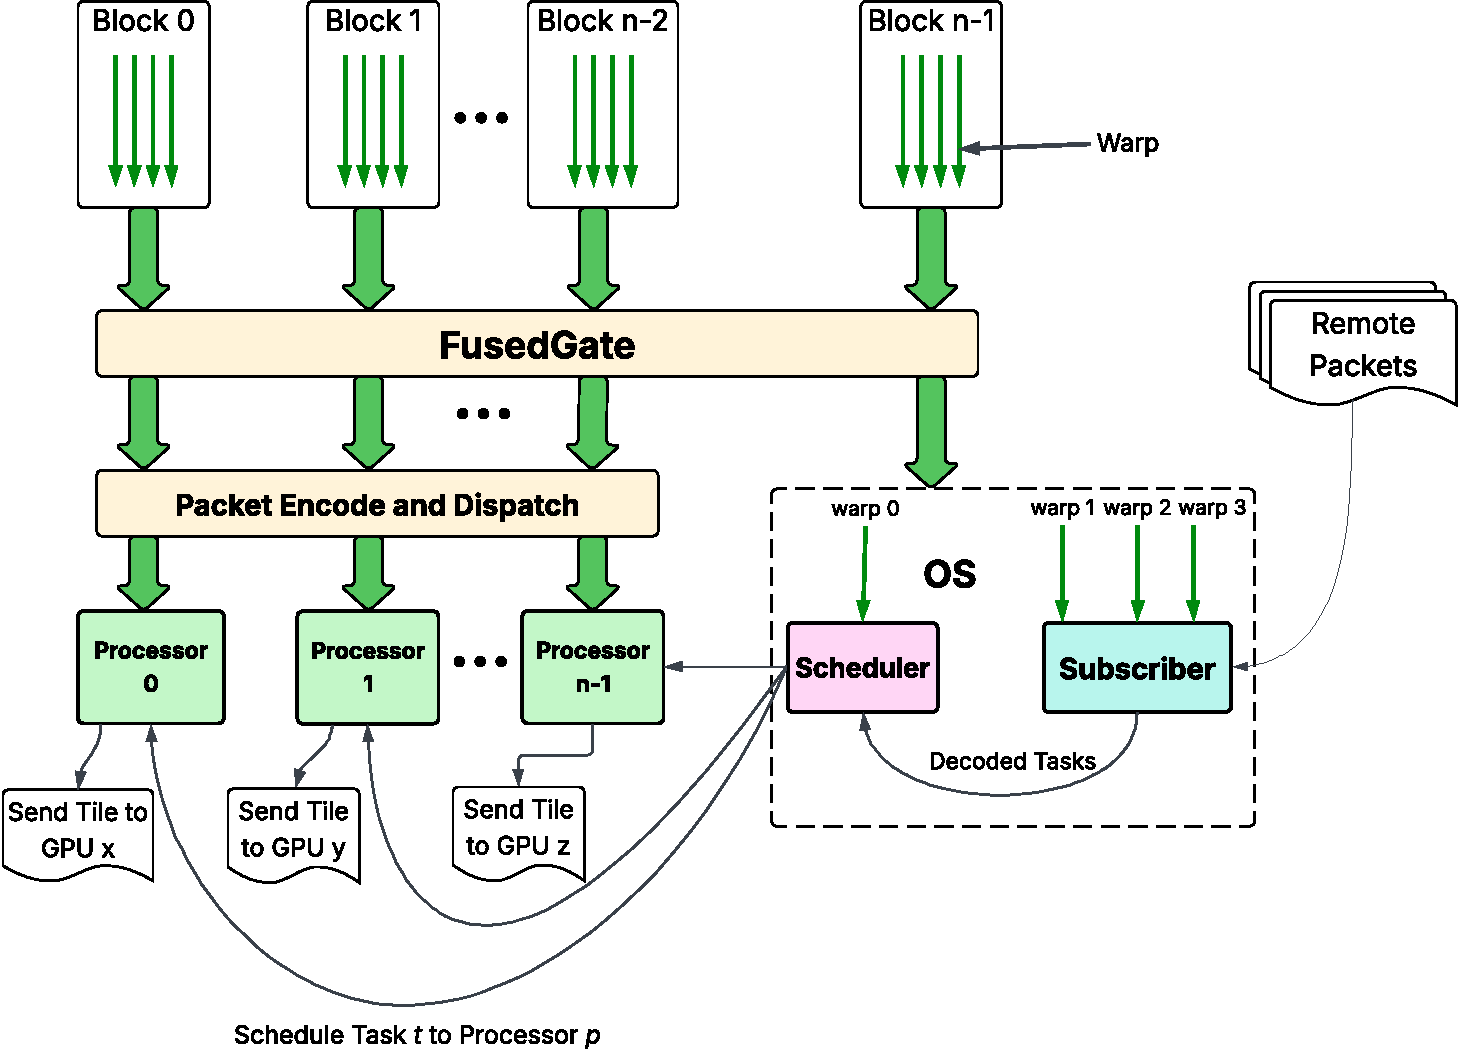
\includegraphics[width=0.8\textwidth, keepaspectratio]{figures/architecture}
    \caption{\emph{\sysname Fused Kernel}. Green arrows demonstrate block or warp specialization.}
    \label{fig:fusedK}
\end{figure}
The performance of modern distributed MoE systems suffers from two primary bottlenecks:
(1) frequent \alltoall collective communication operations on the critical execution path due to expert parallelism,
and (2) significant overhead from repeatedly launching multiple computation and communication kernels on the host CPU.
To overcome these limitations, we introduce \sysname, a fully fused MoE operator implemented as a single persistent GPU kernel.
Unlike previous approaches~\cite{comet, deepep, pmlr-v162-rajbhandari22a, megatron, MLSYS2023_5616d34c,
    MLSYS2024_339caf45, 10.1145/3503221.3508418, 10.1145/3588964, 10.1145/3627703.3650083,
    10.1145/3710848.3710868, NEURIPS2022_67d57c32}, \sysname is the first solution to implement a
\emph{completely fused Distributed MoE kernel}, eliminating kernel launch overhead entirely by
requiring only a single kernel launch (see Table~\ref{tab:gpuOps}).

\SetKwInput{KwRequire}{Require}
\SetKwInput{KwResult}{Result}
\SetKwInput{KwInput}{Input}
\SetKw{kwAnd}{and}
\SetKw{kwOr}{or}
\SetKw{kwTrue}{True}
\SetKw{kwFalse}{False}
\SetKwBlock{DoParallel}{do in parallel}{end}
\begin{algorithm}[!h]
    \DontPrintSemicolon
    \caption{~\emph{\sysname Distributed MoE Fused Kernel}}\label{alg:one}
    \KwInput{$A, O \in \mathbb{R}^{S\times H},\; E \in \mathbb{R}^{L\times H \times P},\; N$}
    \Begin{
        $T, G_{\phi} \gets \mathbf{FusedGate}(A)$\;
        \eIf{blockId $ + 1 < N$}{
            $\mathbf{Dispatch}(T, A)$\;
            processor::start()\;
        }{
            \eIf{$warpID == 0$}{
                scheduler::start()\;
            }{
                subscriber::start($E$, $O$)\;
            }
        }
    }
\end{algorithm}
\section{Actor Model}\label{sec:actor-model}
The design of \sysname is based on the actor model of concurrent
computation~\cite{agha:85, 10.5555/1624775.1624804, Greif:75}.
We implement this model by specializing GPU thread blocks and warps into three distinct actor roles:
(1) \textbf{Processor} (\S\ref{alg:processor}),
(2) \textbf{Subscriber} (\S\ref{alg:susbcriber}),
and (3) \textbf{Scheduler}(\S\ref{alg:scheduler}).
The Processor performs compute (GEMMs and element-wise operations)
and tile communication.
We use CUTLASS~\cite{Thakkar_CUTLASS_2023} as the underlying infrastructure for high-performance
BLAS routines and NVSHMEM for kernel-initiated communication~\cite{nvshm}.
The Subscriber and Scheduler perform administrative functions.
Specifically, the Scheduler assigns computational tasks to available thread blocks.
One key innovation is making the Scheduler both \emph{multithreaded},
enabling high scheduling throughput, and \emph{work-conserving},
ensuring consistently high GPU SM utilization.
On the other hand, the Subscriber subscribes to data communicated over the network.
Of the $N$ thread blocks on a GPU, we specialize $N-1$ to adopt the \textbf{Processor} role.
We specialize the last block for administrative functions.
Within this block, we specialize three warps for the \textbf{Subscriber} role and one warp
for the \textbf{Scheduler} role.
This split of thread blocks across actors is intentional:
our goal is to use few resources for administrative tasks while reserving
bulk of the resources for performing MoE computation tasks.
Figure~\ref{fig:fusedK} summarizes the \sysname architecture and its constituent actors,
while Algorithm~\ref{alg:one} gives a very close translation of the system in code.
\section{Inter-Actor Interactions}\label{sec:inter-actor-interactions}
\begin{figure}[!ht]
    \centering
    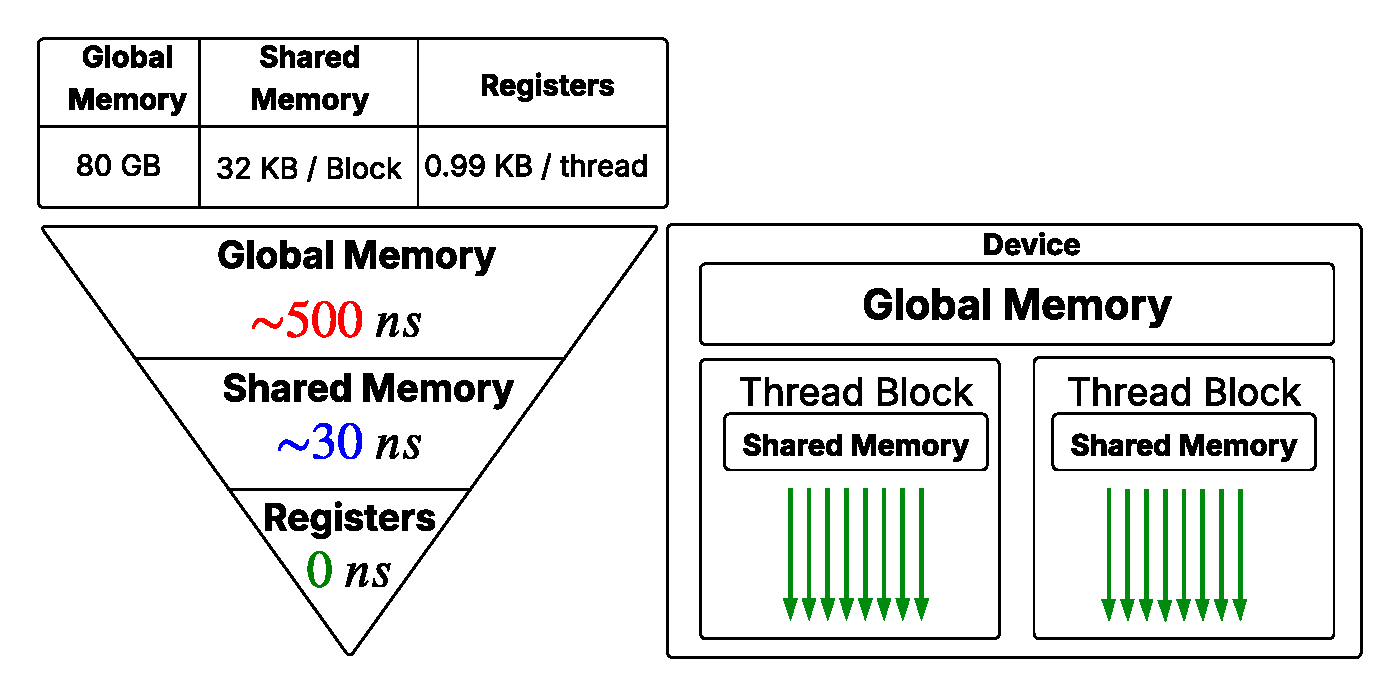
\includegraphics[width=4in, keepaspectratio]{figures/mem}
    \caption{\emph{GPU Memory Hierarchy}.
    The inverted pyramid (left) shows the load/store access latency~\cite{10579250, amperearch, ptx}. Table above outlines the capacity for different memory tiers (for A100 GPUs). The shared memory and register capacity are static configurations for \sysname.
    The right figure shows accessibility scopes: on-chip \textbf{registers}
    are scoped to a thread; on-chip \textbf{shared memory} is visible to all threads in a block;
    and off-chip \textbf{global memory} is accessible by all threads on device.}
    \label{fig:mem}
\end{figure}
\begin{figure}[!ht]
    \centering
    \vspace{-3mm}
    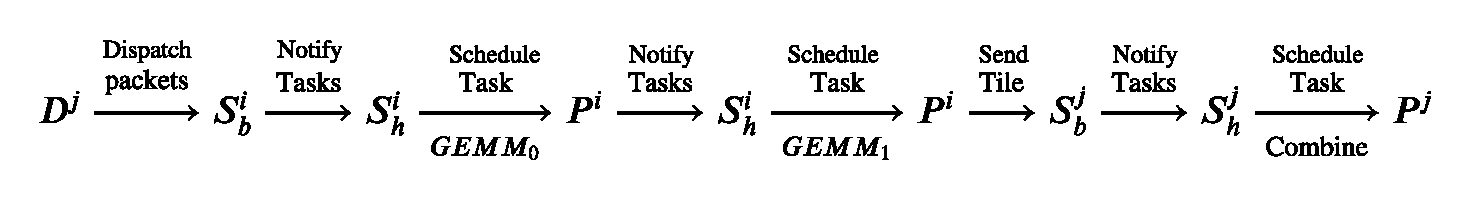
\includegraphics[width=\linewidth]{figures/actors}
    \caption{\emph{DMoE Functional Dependencies Expressed as a Chain of Actor Interactions}.
    We denote $S_b$, $S_h$, and $P$ as the
    Subscriber, Scheduler and Processor actors, respectively. For any actor $a \in \{S_b,\>S_b,\>P\}$,
        $a^i$ identifies an actor on GPU $i$. We define $D^j_i$ as the operator,
        where GPU $j$ dispatches packets of tiles to GPU $i$,
        This diagram expresses task dependencies at the granularity of a tile, namely
        $GEMM_0$, $GEMM_1$, combine and communication produce an output tile.
    }
    \label{fig:actors}
    \vspace{-4mm}
\end{figure}
\sysname decomposes MoE computation and communication at the granularity of a tile,
a statically sized partition of a tensor,
to achieve parallel execution and efficient overlap of tasks.
Each tile corresponds to a discrete unit of work encapsulated by a
\emph{task descriptor}.
The \textbf{Subscriber} actor decodes these
task descriptors from the remote data packets it receives.
Concurrently, the \textbf{Scheduler} actor receives notifications about
available tasks and batches them for execution by the \textbf{Processor} actors.
\textbf{Processor} actors perform computations defined by the tasks,
like the feed-forward network (FFN) and expert-combine operations.
Figure~\ref{fig:actors} shows the chain of actor interactions in \sysname
that comprise DMoE.
\begin{algorithm}[!ht]
    \DontPrintSemicolon
    \SetKwBlock{DoParallel}{do in parallel}{end}
    \caption{~\emph{Subscriber Actor}: executed by three warps}\label{alg:susbcriber}
    \Begin{
        $interrupt \gets \mathbf{GetSharedInterrupt}()$\;
        $flags \gets \mathbf{GetSymmetricFlags}()$\;
        $tQ \gets \mathbf{GetTQ}()$\;
        \tcp{Predefined upper bound on the number of tasks.}
        \tcp{Modulated to the actual task count computed}
        \tcp{from dispatch signals received from peer GPUs}
        $taskBound \gets \mathbf{GetTaskBound}()$\;
        \While{$\mathbf{AtomicLoad}(interrupt) == $ \kwFalse}{
            \tcp{dispatch flags}
            \DoParallel{
                Visit dispatch flags\;
                Atomically retrieve signal\;
                \If{Signal is set and flag is not visited}{
                    Mark visited\;
                    $\mathbf{SelfCorrectTaskBound}(taskBound, Signal)$\;
                    Enforce memory consistency before consuming packet\;
                    Decode packet into a set of $GEMM_0$ task descriptors\;
                    Write task descriptors to $tQ$\;
                    Notify Scheduler of decoded tasks\;
                }
            }
            Advance flags by number of dispatch flags length\;
            Atomically retrieve signal\;
            \tcp{combine signals}
            \DoParallel{
                Visit combine flags: one per tile\;
                \If{Signal is set and flag is not visited}{
                    Mark visited\;
                    Enforce memory consistency before consuming packet\;
                    Decode packet into a set of $combine$ task descriptors\;
                    Write task descriptors to $tQ$\;
                    Notify Scheduler of decoded tasks\;
                }
            }
        }
    }
\end{algorithm}
\begin{algorithm}[!ht]
    \DontPrintSemicolon
    \SetKwInput{KwInput}{Input}
    \SetKwBlock{DoParallel}{do in parallel}{end}
    \KwInput{$N$: Number of processors}
    \caption{~\emph{Scheduler Actor}: executed by one warp}\label{alg:scheduler}
    \Begin{
        $scheduled \gets 0$\;
        $tTB \gets 0$\;
        $tqS \gets \{\}$\;
        $pTDB \gets \mathbf{GetProcessorDoorbell}()$\;
        $sTDB \gets \mathbf{GetSubscriberDoorbell}()$\;
        $taskBound \gets \mathbf{GetTaskBound}()$\;
        $tTB \gets \mathbf{AtomicLoad}(taskBound)$\;
        \tcp{circular buffer ready queue}
        $rQ \gets \{\}$\;
        \tcp{Populate ready queue with Processor ids}
        $\mathbf{PopulateRQ}(rQ)$\;
        \While{$scheduled < tTB$}{
            $lt \gets 0$\;
            \DoParallel{
                Sweep doorbells and populate task counts into $tqS$\;
                Aggregate locally observed task counts into  $lt$\;
            }
            $qS,\>taskTally \gets 0$\;
            \tcp{qS is the inclusive output}
            $\mathbf{WarpInclusiveSum}(lt, qS, tasktally)$\;
            \While{$tasktally > 0$}{
                Repopulate $rQ$ with ready processor ids \;
                \DoParallel{
                    Starting at $rQ[qS]$ signal processors about tasks from $tqS$
                }
            }
            \If{$threadId == 0$}{
                $tTB \gets \mathbf{AtomicLoad}(taskBound)$\;
            }
            $tTB \gets \mathbf{WarpBroadcast}(tTB)$
        }
        $\mathbf{InterruptSubscribers}()$\;
        $\mathbf{InterruptProcessors}()$\;
    }
\end{algorithm}
\begin{algorithm}[!h]
    \DontPrintSemicolon
    \caption{~\emph{Processor Actor}: executed by a block}\label{alg:processor}
    \Begin{
        $tQ \gets \mathbf{GetTQ}()$\;
        $signal \gets 0$\;
        \tcp{shared memory variables}
        $task \gets \{\}$\;
        $interrupt \gets \kwFalse$\;
        $complete \gets \kwFalse$\;
        \While{$interrupt == $ \kwFalse}{
            \If{$warpId == 0$}{
                \If{$threadId == 0$}{
                    $\mathbf{awaitTaskFromScheduler}(interrupt,\>signal)$\;
                    $\mathbf{FencedNotifyRQ}(ready)$\;
                }
                $\mathbf{syncwarp}()$\;
                $\mathbf{warpReadTQ}(tQ, \>signal, \>task)$\;
            }
            $\mathbf{syncthreads}()$\;
            \If{$interrupt == $ \kwFalse}{
                \Switch{task.Type}{
                    \Case{$GEMM_0$}{
                        \tcp{fused GEMM, epilogue and async tile staging}
                        $\mathbf{fGET}(GEMM_0, \>task)$\;
                        \If{$threadId == 0$}{
                            $complete \gets \mathbf{NotifyTileCompletion}()$\;
                        }
                        $\mathbf{syncthreads}()$\;
                        \If{$complete == \kwTrue$}{
                            $\mathbf{NotifySchedulerNextGEMM}(tQ)$\;
                        }
                    }
                    \Case{$GEMM_1$}{
                        \tcp{fused GEMM, epilogue and async tile transfer}
                        $\mathbf{fGET}(GEMM_1, \>task)$\;
                    }
                    \Case{$Combine$}{
                        $\mathbf{combine}(task)$\;
                    }
                }
            }
        }
    }
\end{algorithm}
\section{Tiling}\label{sec:tiling}
Selecting appropriate tile dimensions in \sysname is crucial to ensure efficient GPU utilization.
A small-sized tile underutilizes the GPU's tensor cores,
while excessively large tiles create register pressure,
causing performance-degrading register spills to local memory.
After careful parameter sweeps,
we choose tile dimensions of (128, 64).
Our key insights are: increasing tile width raises the register usage per thread,
potentially triggering costly spills;
increasing tile height without adjusting thread count increases workload per thread, harming performance.
Raising the thread count per block beyond our fixed value of 128 threads reduces the number of concurrent blocks,
negatively affecting SM occupancy.
Larger thread-block sizes also increase overhead from intra-block synchronization (\emph{\_\_syncthreads()} barriers),
further degrading performance.
Thus, our chosen tile dimensions deftly balance these constraints.